\newpage
\subsection{Actividad 10}
Repetir el apartado anterior realizando un diseño de controlador
PID discreto implementable (PD, PI o PID) y ver si es posible cumplir
las especificaciones de sobreoscilación $< 10 \%$, tiempo de
establecimiento test $< 1 s$, error nulo ante ángulo de consigna
escalón unitario y error nulo ante ángulo de consigna rampa unitaria,
graficando la respuesta escalón y rampa, graficando el nuevo lugar de
las raíces en $z$, y comprobando a través de \textsc{ltiview} que se
cumplen ciertamente las especificaciones requeridas.

\begin{tcolorbox}[sharp corners, colframe=bluebox, title= Controlador
  PID con sobreoscilamiento $< 10\%$ y $t_{est} < 1$.,breakable=unlimited]
  $>>>$ rltool(Gposicionz)\\
  \vspace*{0.35em}
  \mkanscode{
\begin{figure}[H]
  \centering
  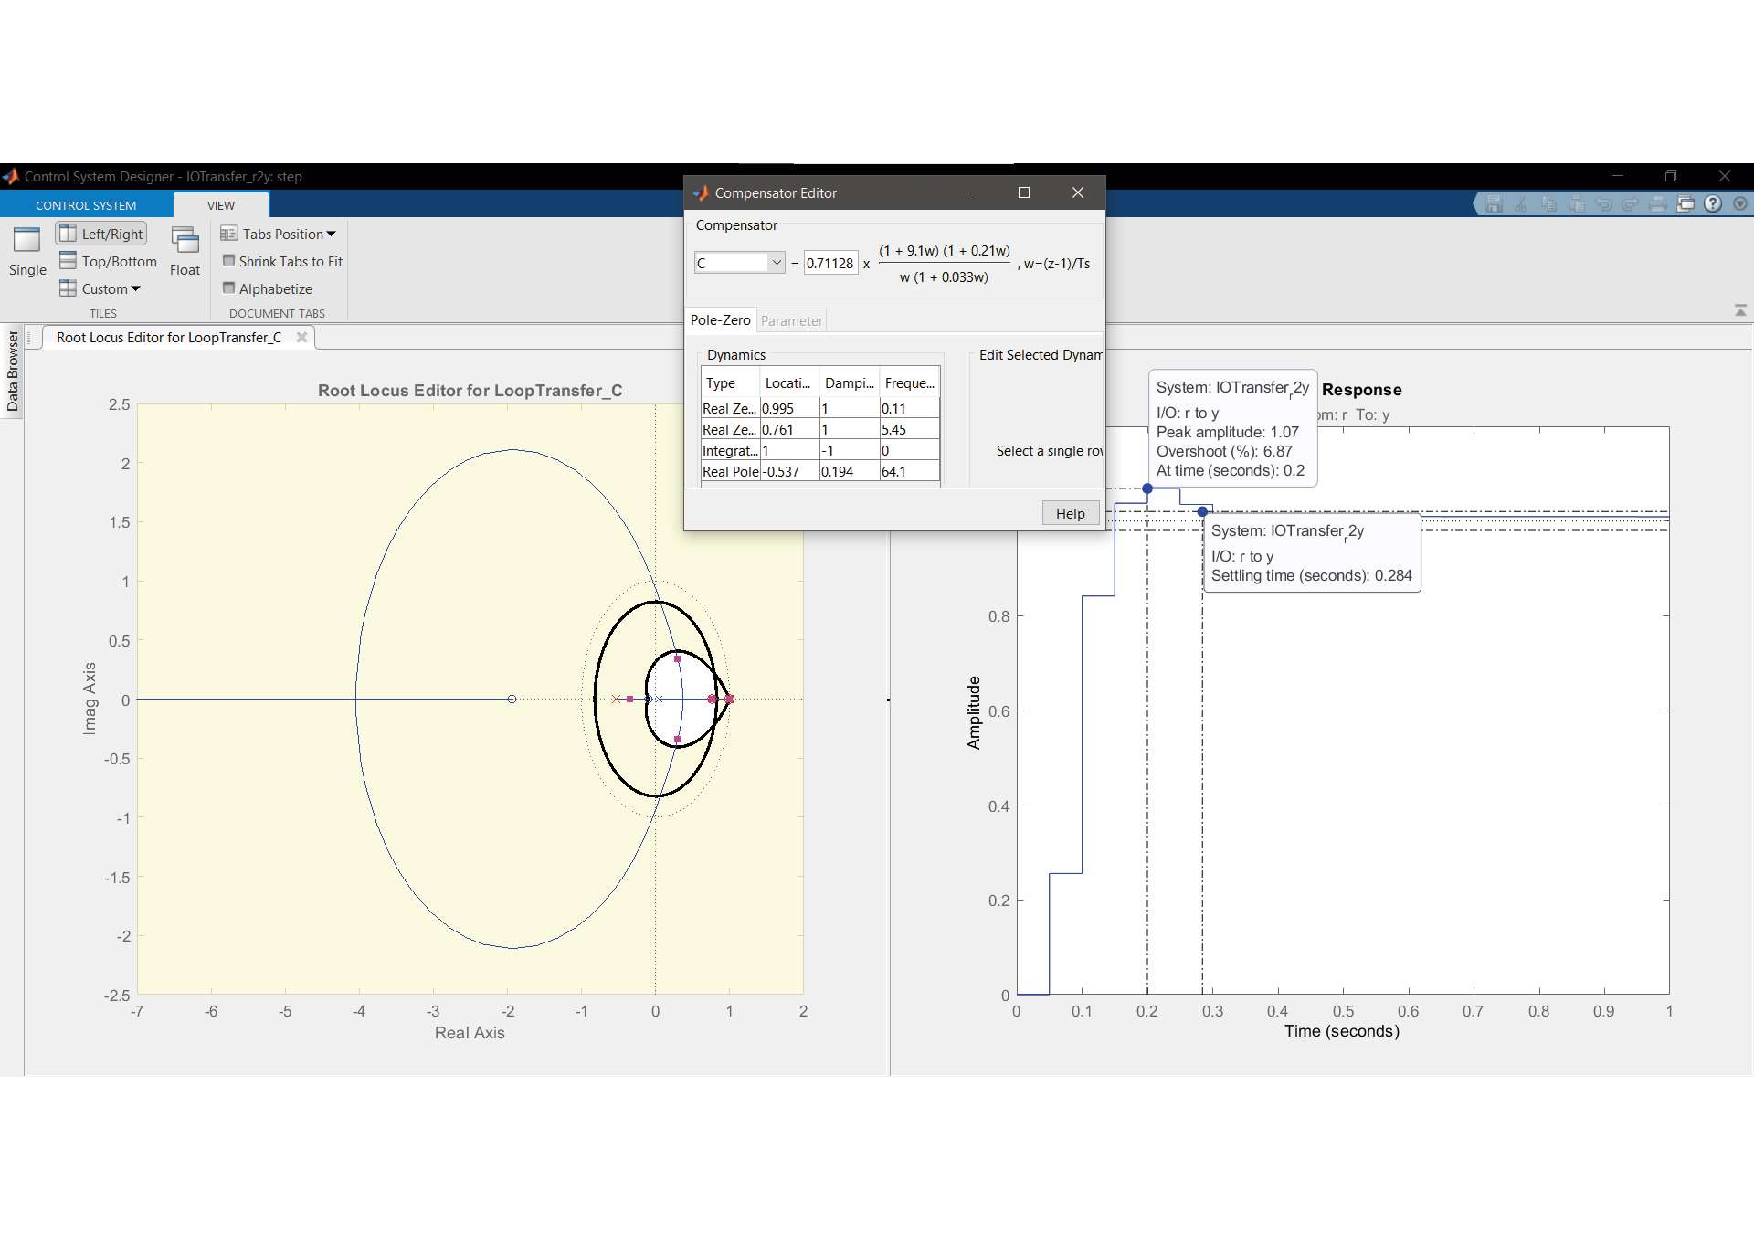
\includegraphics[clip, trim=0cm 2.5cm 0cm 2.5cm,
  scale=0.45]{images/figura 8.pdf}
  % izquierda,abajo,derecha,arriba
  \caption{Controlador PID.}
    \label{fig:figura 8}
\end{figure}
}
\vspace*{0.35em}
Mediante la herramienta \textsc{Export>Export tuned blocks.} podemos
enviar el controlador al espacio de trabajo.

$>>>$ PID\_10
\vspace*{0.35em}
\begin{tcolorbox}[sharp corners, colback = white]
    \color{gray}
\begin{verbatim}
PID_10 =
 
  41.625 (z-0.9945) (z-0.7613)
  ----------------------------
        (z-1) (z+0.5366)
 
Sample time: 0.05 seconds
Discrete-time zero/pole/gain model.
\end{verbatim}
  \end{tcolorbox}%
  \vspace*{0.5em}
\end{tcolorbox}%

\begin{tcolorbox}[sharp corners, colframe=bluebox, title= Respuesta
  del sistema en tiempo discreto con un controlador PID.]
  $>>>$ ltiview(\textcolor{blue}{`step'},kr*feedback(PID\_10*Gposicionz,kr))
  \vspace*{0.35em}
  \mkanscode{
\begin{figure}[H]
  \centering
  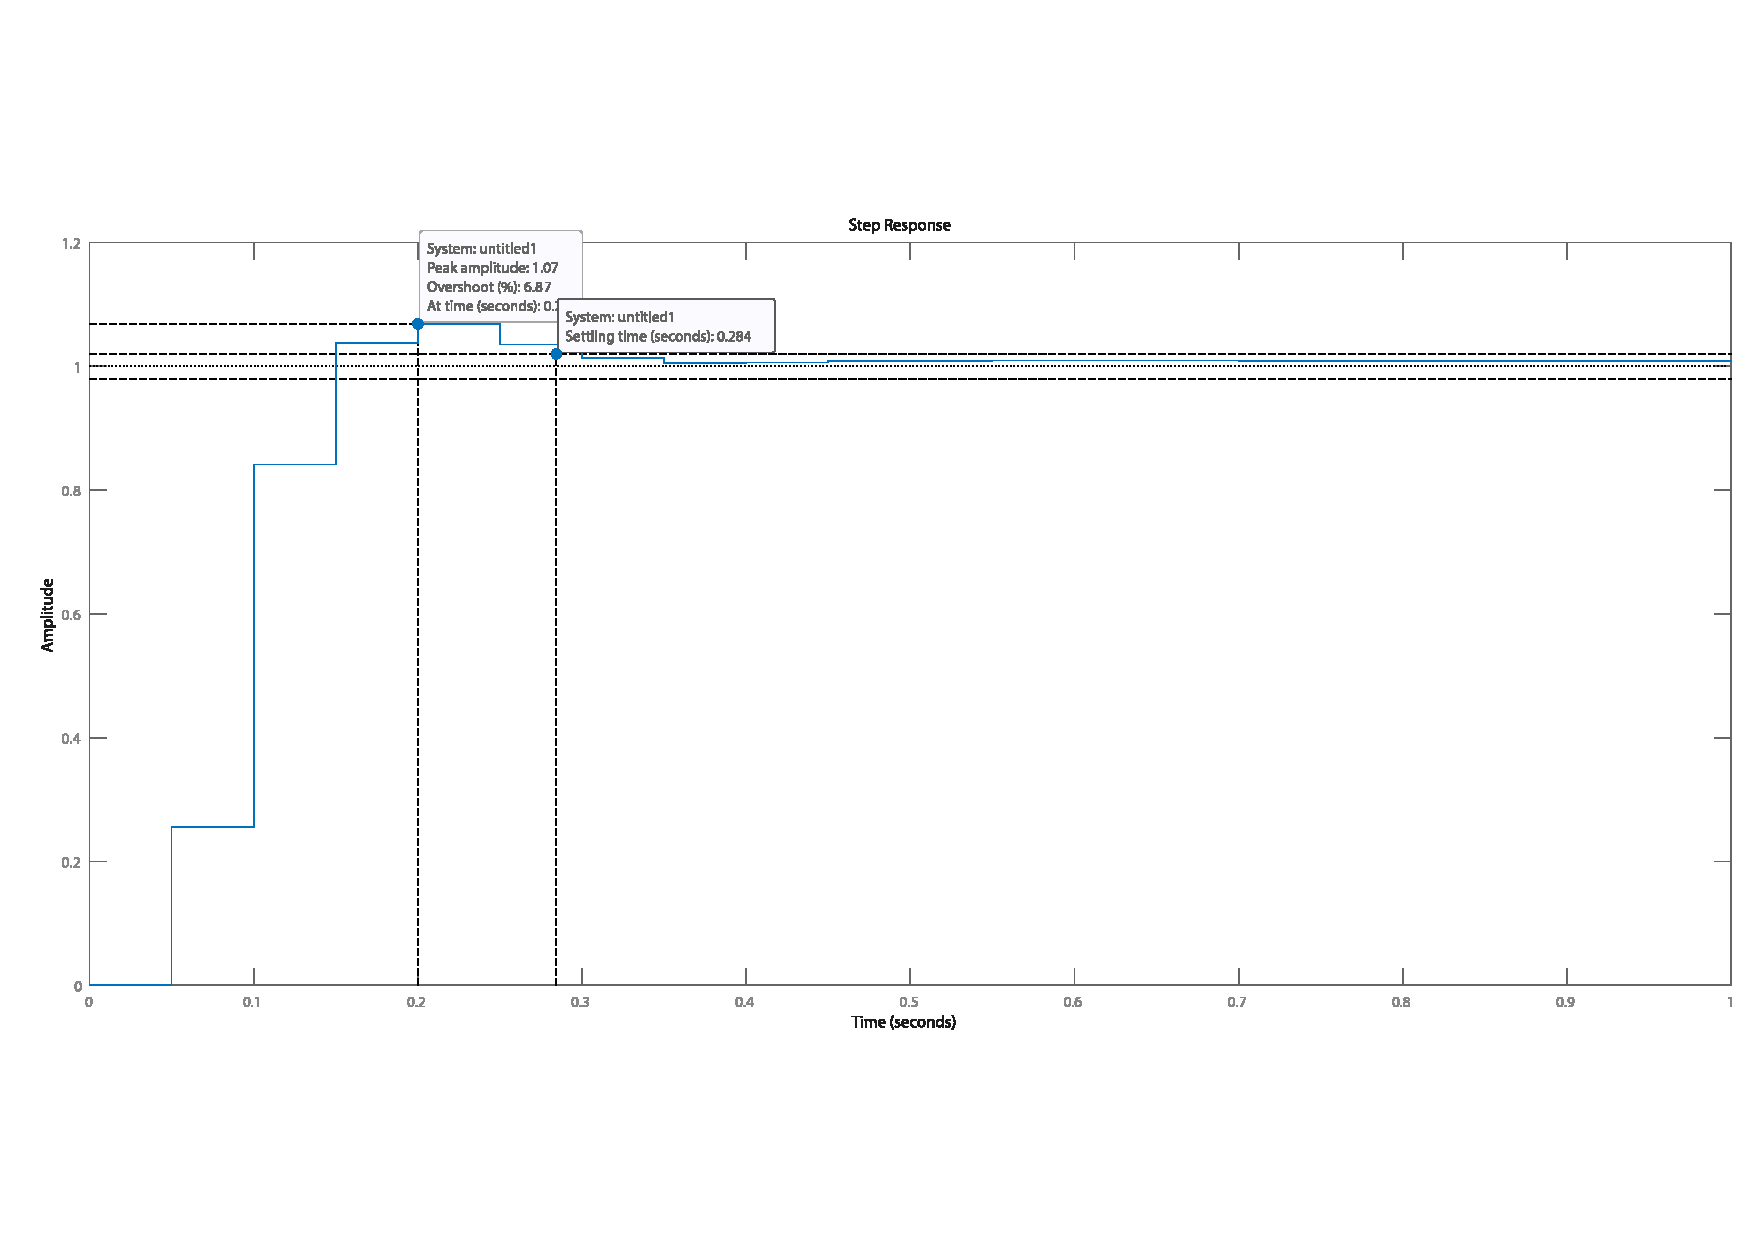
\includegraphics[clip, trim=0cm 3.6cm 0cm 3.4cm,scale=0.45]{images/figura 9.pdf}
  % izquierda,abajo,derecha,arriba
  \caption{Respuesa del sistema frente a un escalón con un controlador PID.}
    \label{fig:figura 9}
\end{figure}
}

\end{tcolorbox}%

\begin{tcolorbox}[sharp corners, colframe=bluebox, title= Respuesta
  del sistema en tiempo discreto con un controlador PID.]
  $>>>$ ltiview(\textcolor{blue}{`lsim'},kr*feedback(PID\_10*Gposicionz,kr))
  \vspace*{0.35em}
  \mkanscode{
\begin{figure}[H]
  \centering
  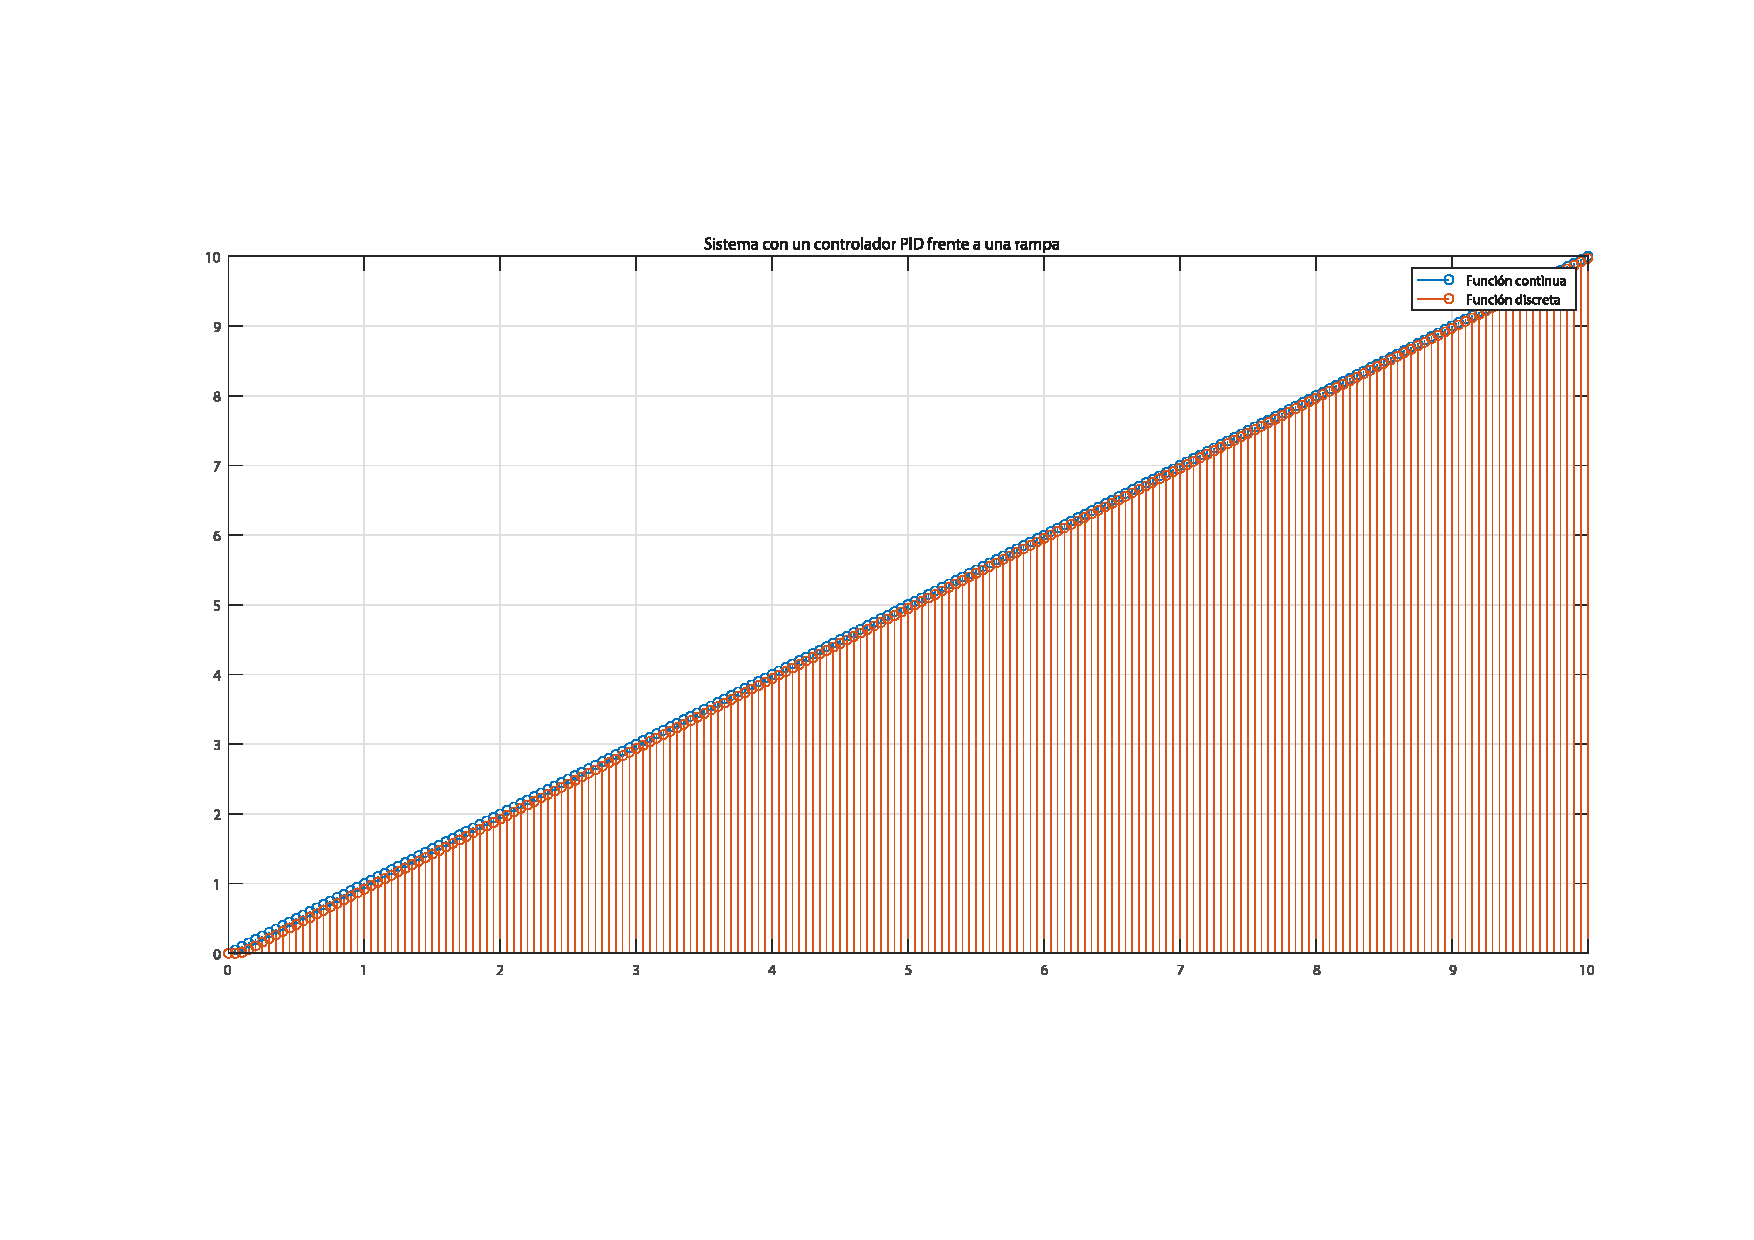
\includegraphics[clip, trim=2cm 3.6cm 1.4cm 3.4cm,scale=0.48]{images/figura 10.pdf}
  % izquierda,abajo,derecha,arriba
  \caption{Respuesa del sistema frente a una rampa con un controlador PID.}
    \label{fig:figura 10}
\end{figure}
}

\end{tcolorbox}%